\chapter{Botten en spieren}\label{ch:g3:bones-and-muscles}

Spring, en land: iets in je heeft zojuist als een volmaakte machine
gewerkt. Stevige staven hielden je vorm vast, scharnieren lieten je
\omterm{def:g1:my-body:parts}{benen} vouwen en \omterm{def:g1:animals-around-us:covering}{veren}, en honderden kleine motoren trokken precies op
het juiste moment. De staven zijn je \omterm{def:g3:bones-and-muscles:skeleton}{botten}, de scharnieren je
\omterm{prop:g3:bones-and-muscles:joints}{gewrichten}, de motoren je \omterm{def:g3:bones-and-muscles:muscle}{spieren} --- de uitrusting van het lichaam
voor elke beweging die het ooit zal maken.

\section{Het skelet}

\begin{definition}[Skelet en botten]\label{def:g3:bones-and-muscles:skeleton}
Het \emph{skelet}\index{skelet} is het geraamte van ongeveer $200$
\emph{botten}\index{bot} in het lichaam. De belangrijkste delen:
\begin{itemize}
  \item de \emph{schedel}\index{schedel}, een stevige helm van bot om
        de hersenen heen;
  \item de \emph{wervelkolom}\index{wervelkolom} (ruggengraat), een
        buigzame zuil van kleine botjes gestapeld van nek tot heupen,
        die de \omterm{def:g1:my-body:parts}{romp} rechtop houdt;
  \item de \emph{ribben}\index{rib}, gebogen botten die een kooi om
        hart en longen vormen;
  \item de \emph{pijpbeenderen}: lange botten in \omterm{def:g1:my-body:parts}{armen} en \omterm{def:g1:my-body:parts}{benen} --- het
        dijbeen is het langste van het lichaam.
\end{itemize}
\end{definition}

\begin{omfigure}
\begin{tikzpicture}
  \node[anchor=south west, inner sep=0] (img) at (0,0)
    {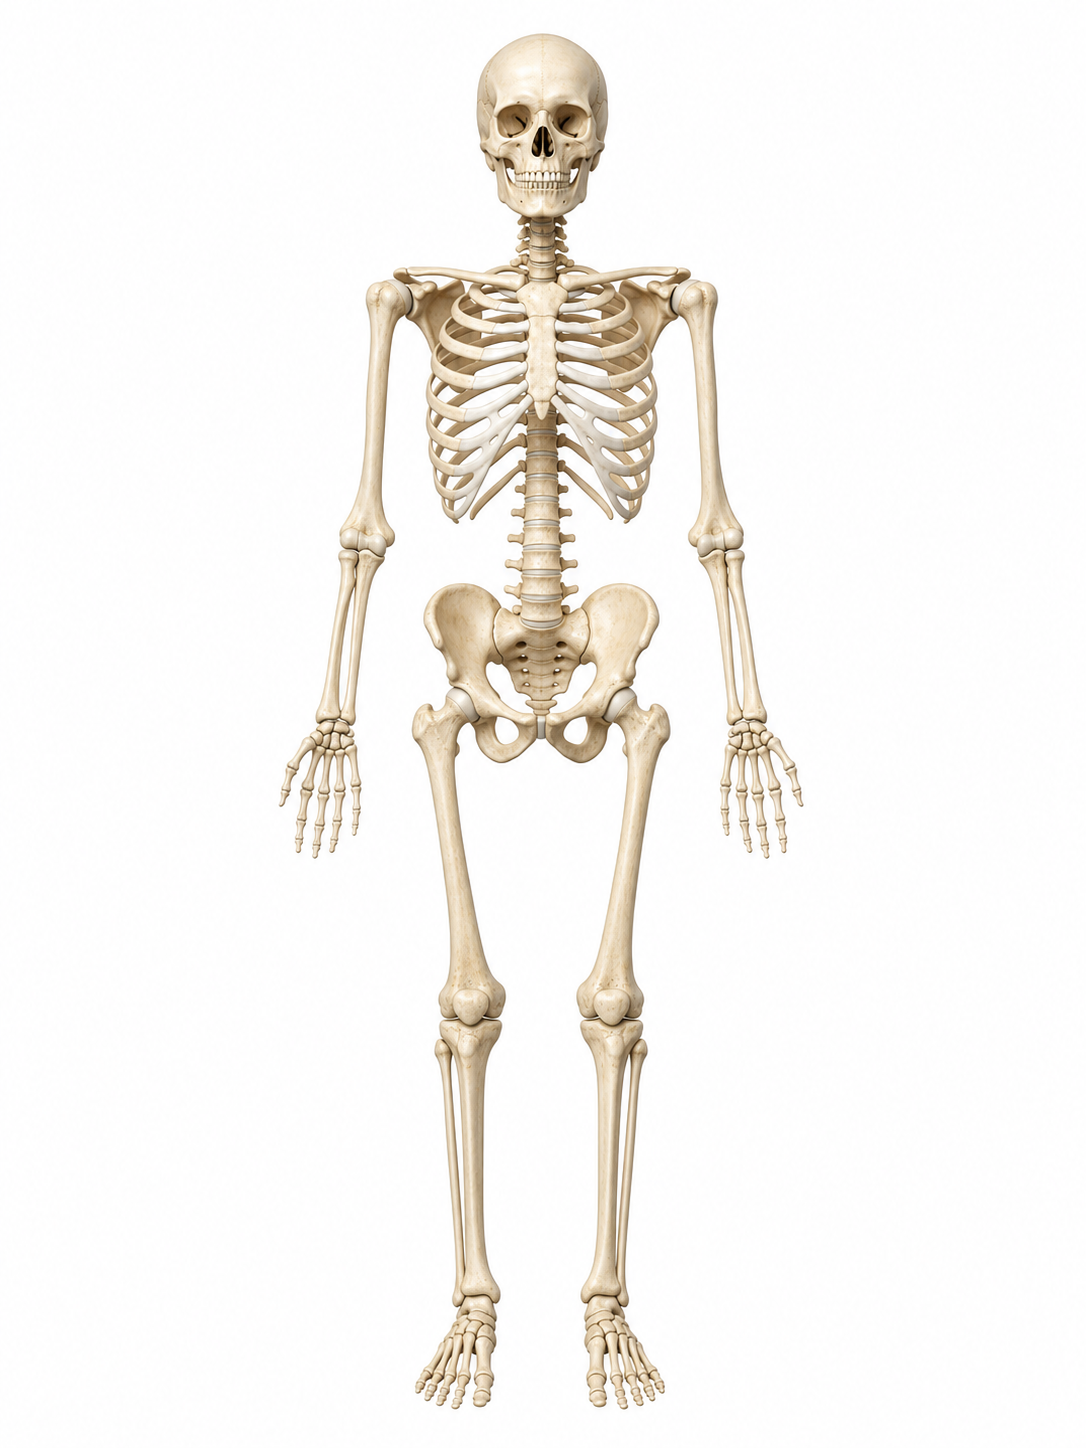
\includegraphics[width=0.46\linewidth]{images/book1/ai/fig-skeleton.png}};
  \begin{scope}[x={(img.south east)}, y={(img.north west)},
      every node/.style={font=\small}]
    \draw[omDef, thick] (0.56,0.93) -- (0.72,0.95) node[right] {schedel};
    \draw[omDef, thick] (0.40,0.73) -- (0.20,0.82)
      node[above, align=center] {ribben: een kooi voor\\ hart en longen};
    \draw[omDef, thick] (0.52,0.56) -- (0.72,0.60)
      node[right, align=left] {wervelkolom: gestapelde\\ botjes};
    \draw[omDef, thick] (0.60,0.36) -- (0.76,0.38) node[right] {dijbeen};
    \draw[omThm, thick] (0.335,0.615) circle (0.022);
    \draw[omThm, thick] (0.445,0.265) circle (0.022);
    \draw[omThm, thick] (0.425,0.265) -- (0.20,0.22)
      node[left, align=center, omThm] {gewrichten (in rood):\\ waar botten elkaar raken};
  \end{scope}
\end{tikzpicture}

{\small Het bouwplan van het \omterm{def:g3:bones-and-muscles:skeleton}{skelet}: helm, zuil, kooi en lange \omterm{def:g3:bones-and-muscles:skeleton}{botten}
in de \omterm{def:g1:my-body:parts}{ledematen} die elkaar in \omterm{prop:g3:bones-and-muscles:joints}{gewrichten} raken.}
\end{omfigure}

\begin{example}[Voel je geraamte]\label{ex:g3:bones-and-muscles:feel}
Geen röntgenfoto nodig: druk voorzichtig en het \omterm{def:g3:bones-and-muscles:skeleton}{skelet} meldt zich.
Knokkels; de rand van je scheenbeen; de ketting van kleine bobbels
midden over je rug --- de \omterm{def:g3:bones-and-muscles:skeleton}{wervelkolom}, botje na botje; de \omterm{def:g3:bones-and-muscles:skeleton}{ribben} die je
onder je vingers kunt tellen. Het geraamte zit vlak onder de \omterm{def:g1:the-five-senses:sense}{huid}.
\end{example}

\begin{remark}[Hard van buiten, levend van binnen]\label{rem:g3:bones-and-muscles:alive}
Een \omterm{def:g3:bones-and-muscles:skeleton}{bot} is geen dood materiaal zoals een stukje krijt: het leeft, het
wordt door bloed gevoed, het groeit terwijl jij groeit --- en het kan
zichzelf herstellen. Een gebroken \omterm{def:g1:my-body:parts}{arm} in het gips geneest doordat het
\omterm{def:g3:bones-and-muscles:skeleton}{bot} zelf de breuk langzaam opnieuw opbouwt. Krijtjes doen dat nooit.
\end{remark}

\begin{omfigure}
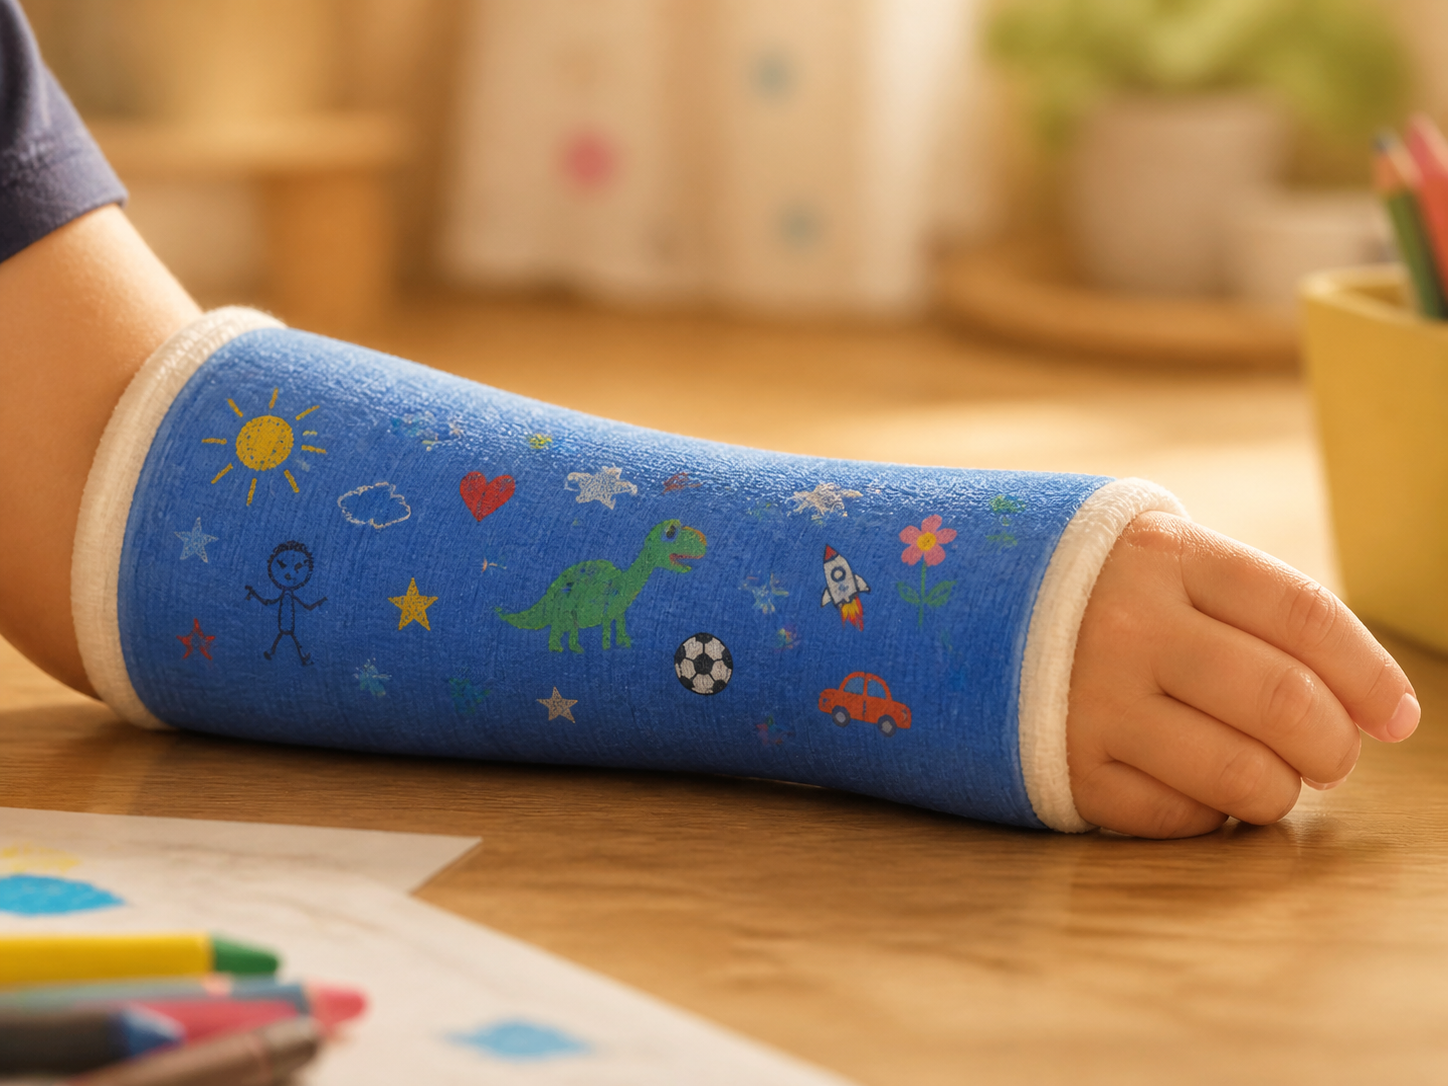
\includegraphics[width=0.56\linewidth]{images/book1/ai/g3-bones-cast.png}

{\small In het beschilderde gips, stil gehouden, bouwt een levend \omterm{def:g3:bones-and-muscles:skeleton}{bot}
zichzelf in alle rust weer op.}
\end{omfigure}

\section{Gewrichten, waar het geraamte buigt}

\begin{proposition}[Stevige staven, buigplekken]\label{prop:g3:bones-and-muscles:joints}
\omterm{def:g3:bones-and-muscles:skeleton}{Botten} zelf buigen nooit --- een gebogen \omterm{def:g3:bones-and-muscles:skeleton}{bot} is een gebroken \omterm{def:g3:bones-and-muscles:skeleton}{bot}. Al
het buigen van het lichaam gebeurt in de
\emph{gewrichten}\index{gewricht}, waar twee \omterm{def:g3:bones-and-muscles:skeleton}{botten} elkaar raken:
\omterm{def:g1:my-body:joint}{schouder}, \omterm{def:g1:my-body:joint}{elleboog}, \omterm{def:g1:my-body:joint}{pols}, heup, \omterm{def:g1:my-body:joint}{knie}, enkel, en de vele kleine
\omterm{prop:g3:bones-and-muscles:joints}{gewrichten} van de \omterm{def:g3:bones-and-muscles:skeleton}{wervelkolom}, waarvan de kleine buigingen bij elkaar
een soepele rug opleveren.
\end{proposition}
\admitted

\begin{example}[De truc van de wervelkolom]\label{ex:g3:bones-and-muscles:spinetrick}
Geen enkel \omterm{def:g3:bones-and-muscles:skeleton}{bot} in je rug kan krullen --- en toch kun je je bijna tot
een bal voorover rollen. De \omterm{def:g3:bones-and-muscles:skeleton}{wervelkolom} is een zuil van meer dan $20$
botjes, die elk een paar graden op hun buren draaien: veel kleine
buigingen die samen één grote maken. Daarom moet je ook je knieën
buigen en niet je rug om iets zwaars op te tillen --- knieën zijn
gebouwd voor grote vouwen, de \omterm{def:g3:bones-and-muscles:skeleton}{wervelkolom} voor zachte.
\end{example}

\section{Spieren, de bewegers}

\begin{definition}[Spier]\label{def:g3:bones-and-muscles:muscle}
Een \emph{spier}\index{spier} is een vlezige motor die aan de \omterm{def:g3:bones-and-muscles:skeleton}{botten}
vastzit. Een spier kan \emph{samentrekken}\index{samentrekken} ---
korter en dikker worden --- en door samen te trekken \emph{trekt} hij
aan het \omterm{def:g3:bones-and-muscles:skeleton}{bot} waaraan hij vastzit. Spieren trekken alleen; geen enkele
spier kan duwen.
\end{definition}

\begin{proposition}[Werken in paren]\label{prop:g3:bones-and-muscles:pairs}
Omdat \omterm{def:g3:bones-and-muscles:muscle}{spieren} alleen trekken, is er voor het twee kanten op bewegen van
een \omterm{def:g1:my-body:joint}{gewricht} een \emph{paar} nodig: één \omterm{def:g3:bones-and-muscles:muscle}{spier} aan de voorkant van de
\omterm{def:g1:my-body:parts}{arm} buigt de \omterm{def:g1:my-body:joint}{elleboog}, zijn partner aan de achterkant strekt hem; elk
ontspant terwijl de ander trekt. Bijna elk \omterm{def:g1:my-body:joint}{gewricht} van het lichaam
wordt door zulke paren bewogen.
\end{proposition}
\admitted

\begin{omfigure}
\begin{tikzpicture}
  \node[anchor=south west, inner sep=0] (img) at (0,0)
    {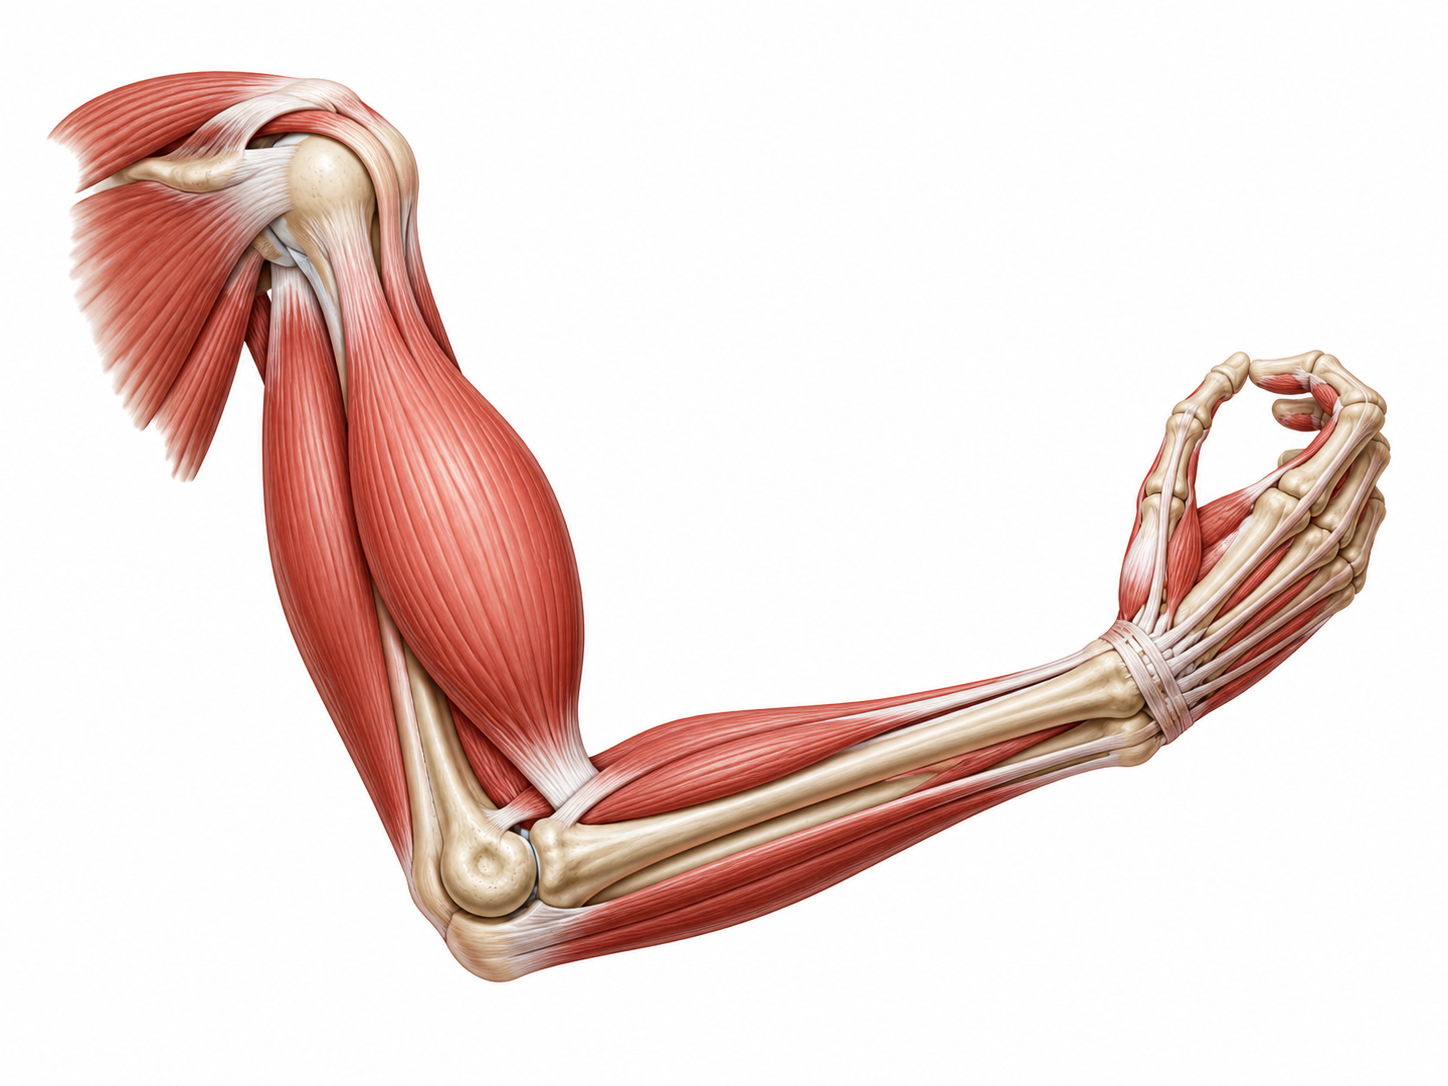
\includegraphics[width=0.62\linewidth]{images/book1/ai/fig-arm-muscles.png}};
  \begin{scope}[x={(img.south east)}, y={(img.north west)},
      every node/.style={font=\small}]
    \draw[omThm, thick] (0.42,0.58) -- (0.58,0.78)
      node[right, align=left, omThm]
      {de voorste spier, bollend:\\ hij trekt samen en trekt};
    \draw[omDef, thick] (0.23,0.46) -- (0.14,0.22)
      node[below, align=center, omDef]
      {de achterste spier\\ van het paar, in rust};
  \end{scope}
\end{tikzpicture}

{\small De \omterm{def:g1:my-body:joint}{elleboog} buigen: de voorste \omterm{def:g3:bones-and-muscles:muscle}{spier} van het paar bolt op
terwijl hij korter wordt en de onderarm omhoogtrekt, terwijl zijn
partner erachter rust. Om te strekken wisselen de twee van rol.}
\end{omfigure}

\begin{example}[Voel het paar aan het werk]\label{ex:g3:bones-and-muscles:pair}
Pak je bovenarm met je andere hand vast en buig langzaam je \omterm{def:g1:my-body:joint}{elleboog}:
de \omterm{def:g3:bones-and-muscles:muscle}{spier} aan de voorkant zwelt op en wordt hard --- hij trekt samen.
Strek nu je \omterm{def:g1:my-body:parts}{arm}: de voorkant wordt zacht, en achter de \omterm{def:g1:my-body:parts}{arm} spant zijn
partner juist aan. Je hebt zojuist
\cref{prop:g3:bones-and-muscles:pairs} zelf gevoeld.
\end{example}

\begin{method}[Voor botten en spieren zorgen]\label{met:g3:bones-and-muscles:care}
\begin{enumerate}
  \item Beweeg elke dag --- \omterm{def:g3:bones-and-muscles:skeleton}{botten} worden door gebruik sterker, \omterm{def:g3:bones-and-muscles:muscle}{spieren} ook;
  \item eet het voedsel van de bouwers: zuivel voor de \omterm{def:g3:bones-and-muscles:skeleton}{botten}, en
        gevarieerde maaltijden (\cref{ch:g2:teeth-and-eating-well});
  \item warm op vóór zwaar sporten, zodat \omterm{def:g3:bones-and-muscles:muscle}{spieren} rekken in plaats van
        scheuren;
  \item til zware dingen op met gebogen knieën en een rechte rug;
  \item helm en beschermers waar vallen waarschijnlijk is: \omterm{def:g3:bones-and-muscles:skeleton}{botten}
        herstellen, maar langzaam.
\end{enumerate}
\end{method}

\section{Oefeningen}

\begin{exercise}[$\star$]\label{exo:g3:bones-and-muscles:1}
Noem de vier delen van het \omterm{def:g3:bones-and-muscles:skeleton}{skelet} uit
\cref{def:g3:bones-and-muscles:skeleton}, en wat elk beschermt of
overeind houdt.
\end{exercise}

\begin{exercise}[$\star$]\label{exo:g3:bones-and-muscles:2}
Ongeveer hoeveel \omterm{def:g3:bones-and-muscles:skeleton}{botten} heeft het \omterm{def:g3:bones-and-muscles:skeleton}{skelet}? Welk \omterm{def:g3:bones-and-muscles:skeleton}{bot} is het langste?
\end{exercise}

\begin{exercise}[$\star$]\label{exo:g3:bones-and-muscles:3}
Kan een \omterm{def:g3:bones-and-muscles:skeleton}{bot} buigen? Waar gebeurt al het buigen van het lichaam?
\end{exercise}

\begin{exercise}[$\star$]\label{exo:g3:bones-and-muscles:4}
De \omterm{def:g3:bones-and-muscles:skeleton}{wervelkolom} kan krullen hoewel geen van haar \omterm{def:g3:bones-and-muscles:skeleton}{botten} dat kan. Leg
haar truc uit.
\end{exercise}

\begin{exercise}[$\star$]\label{exo:g3:bones-and-muscles:5}
Wat doet een \omterm{def:g3:bones-and-muscles:muscle}{spier} als hij samentrekt? Wat kan geen enkele \omterm{def:g3:bones-and-muscles:muscle}{spier} ooit?
\end{exercise}

\begin{exercise}[$\star$]\label{exo:g3:bones-and-muscles:6}
Waarom zijn er voor het buigen en strekken van de \omterm{def:g1:my-body:joint}{elleboog} twee \omterm{def:g3:bones-and-muscles:muscle}{spieren}
nodig? Vertel wat elk op elk moment doet.
\end{exercise}

\begin{exercise}[$\star$]\label{exo:g3:bones-and-muscles:7}
Hoe geneest een gebroken \omterm{def:g1:my-body:parts}{arm} in het gips? Wat laat dat over \omterm{def:g3:bones-and-muscles:skeleton}{bot} zien,
volgens \cref{rem:g3:bones-and-muscles:alive}?
\end{exercise}

\begin{exercise}[$\star$]\label{exo:g3:bones-and-muscles:8}
Probeer het: doe de greeptest van \cref{ex:g3:bones-and-muscles:pair}
op je eigen \omterm{def:g1:my-body:parts}{arm}. Beschrijf wat de voorkant van je \omterm{def:g1:my-body:parts}{arm} doet als je
buigt, en als je strekt.
\end{exercise}

\begin{exercise}[$\star\star$]\label{exo:g3:bones-and-muscles:9}
Waarom zeggen volwassenen ``til met je knieën, niet met je rug''?
Antwoord met \cref{ex:g3:bones-and-muscles:spinetrick}.
\end{exercise}

\begin{exercise}[$\star\star$]\label{exo:g3:bones-and-muscles:10}
Een marionet aan touwtjes kun je laten zwaaien: elk touwtje kan zijn
\omterm{def:g1:my-body:parts}{arm} maar één kant op \emph{trekken}. Hoe is dat precies de situatie van
de \omterm{def:g3:bones-and-muscles:muscle}{spieren}, en wat is het antwoord van de poppenmaker daarop? Vergelijk
met \cref{prop:g3:bones-and-muscles:pairs}.
\end{exercise}
